\chapter{Конструкторский раздел}
\label{cha:design}

В данном разделе на основе проведенного анализа описывается взаимодействие между подсистемами, выделяются основные составляющие в каждой системе и проектируется их взаимодействие.

% \section{Конструкция робота}


\section{Подсистема распознавания}
\subsection{Основные задачи}
В данной секции сформируем опишем уже формализованный список задач, которые нам необходимо будет произвести над картинкой.
Модно выделить основные моменты при данной системой:
\begin{enumerate}
  \item сфотографировать;
  \item перевести изображение в черно-белые цвета;
  \item определить угол наклона изображения;
  \item определить сетку;
  \item распознать и разместить цифры в сетке;
  \item скорректировать распознавание под правила Судоку.
\end{enumerate}

\subsection{Фотографирование}
Данный процесс делается стандартными средствами Android API. Необходимо лишь получить изображение из камеры или галереи, после чего передать изображение на обработку.

\subsection{Конвертация в монохромное изображение}
Каждое приложение с компьютерным зрением начинает с конвертации цветного (или чёрно-белого) изображения в монохромное. В будущем, возможно, будет какой-то алгоритм, который будет использовать цвета, но сегодня приложения компьютерного зрения работают с монохромными изображениями (они дальтоники).
Самый простой метод для конвертации изображения – это общий порог. Предположим, что у вас есть пиксель с цветом RGB (200, 200, 200). Так как интенсивность компонент изменяется от 0 до 255, то пиксель очень яркий. Выбрав порог, как половину интенсивности: 256/2=128, мы получим, что наш пиксель должен стать белым. Но общий порог редко используется в настоящих приложениях, так как он малополезен. Куда более полезен алгоритм локального порога.

На рис.~\ref{fig:fig21} показаны оригинальное фото (1), фото после обработки с общим порогом (2) и адаптивным порогом (3) .

\begin{figure}[ht!]
  \centering
  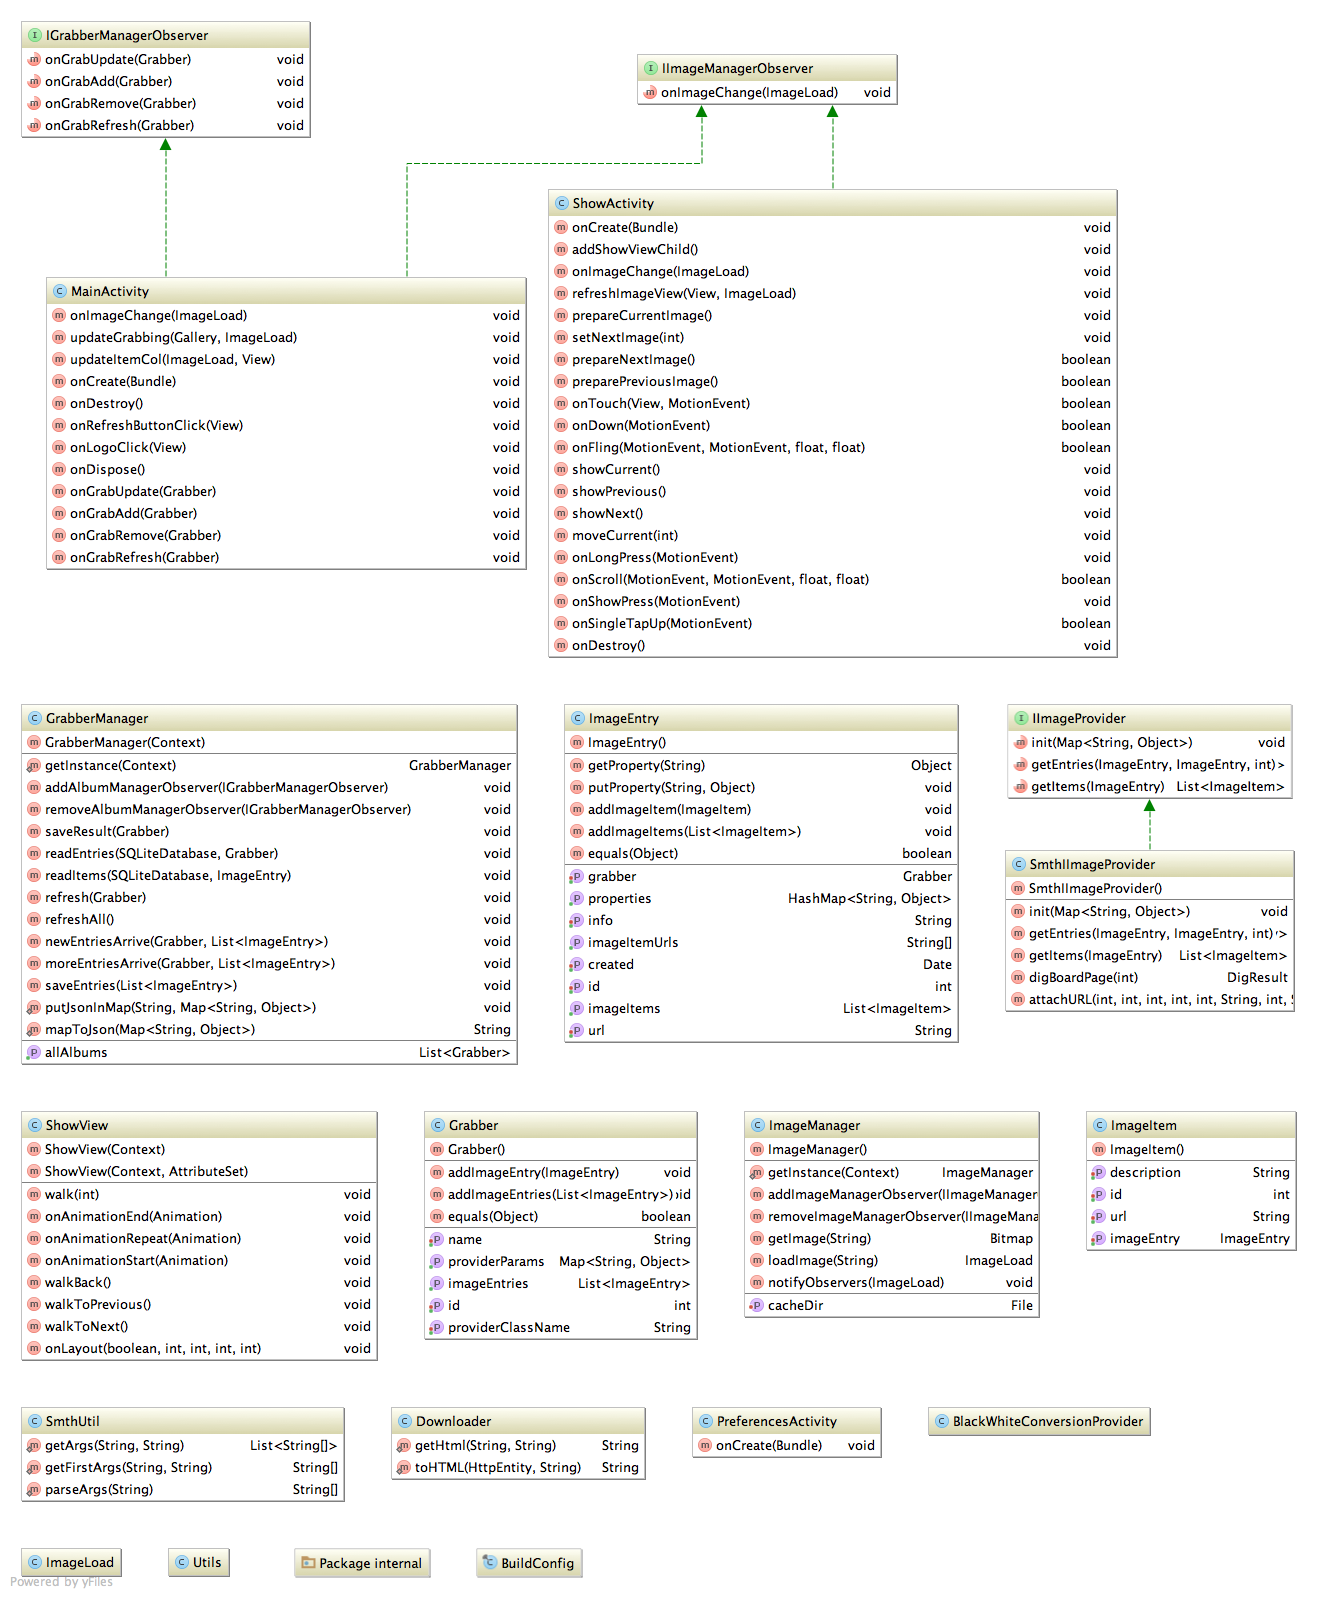
\includegraphics[width=\textwidth]{inc/raster/design2-1.png}
  \caption{Пороги при создании монохромного изображения}
  \label{fig:fig21}
\end{figure}

Для правильной конвертации изображения в монохромное, мы будем использовать адаптивный выбор порога. Он не использует фиксированное значение порога в 128. Вместо этого, он считает порог для каждого пикселя отдельно. Он берёт квадрат со стороной в ${l}$ пикселей и с центром в нашем пикселе и суммирует интенсивность всех точек. Среднее значение интенсивности и будет являться порогом для данного пикселя. Формула интенсивности для текущего пикселя: $\text{порог}=\frac{\text{сумма}}{l^2}$. Если интенсивность нашего пикселя выше порогового значения, то он конвертируется в белый, если же нет, то в чёрный. На изображении ниже пиксель, для которого определяется порог, отмечен красным. И эти подсчёты производятся для каждого пикселя. Поэтому данный шаг является таким медленным, ведь алгоритм требует $\text{ширина} * \text{порог} *{l^2}$ чтений пикселя изображения. Схема показана на рис.~\ref{fig:fig22}

\begin{figure}[ht!]
  \centering
  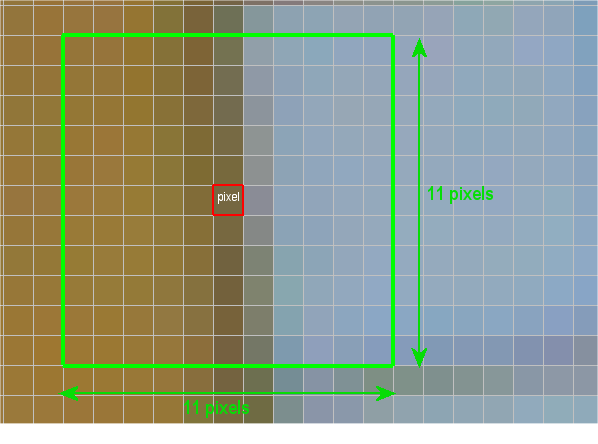
\includegraphics[width=0.7\textwidth]{inc/raster/design2-2.png}
  \caption{Адаптивный выбор порога при создании монохромного изображения}
  \label{fig:fig22}
\end{figure}

\subsubsection{Целочисленная форма}
\begin{figure}[ht!]
  \centering
  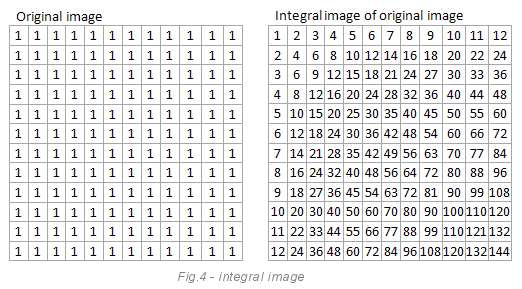
\includegraphics[width=\textwidth]{inc/raster/design2-3.png}
  \caption{Целочисленная форма}
  \label{fig:fig23}
\end{figure}

Этот шаг может быть оптимизирован с помощью использования «Целочисленной формы». Целочисленная форма – это массив целых чисел с размерами изображения. Допустим у нас есть область  на рис.~\ref{fig:fig23} $12{*}12$, где интенсивность пикселей равна $1$ (в реальном мире так не бывает), целочисленный образ – это сумма всех пикселей с левого верхнего до текущего (правого нижнего).

\begin{figure}[ht!]
  \centering
  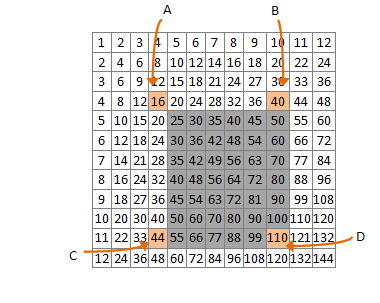
\includegraphics[width=0.6\textwidth]{inc/raster/design2-4.png}
  \caption{Целочисленная форма в области}
  \label{fig:fig24}
\end{figure}
Следующий рис.~\ref{fig:fig24} демонстрирует, чем может быть полезен целочисленный образ. Целью является посчитать сумму пикселей в сером прямоугольнике. 
Формула: $\text{сумма}=D{-}C{-}B{+}A$ . В нашем случае: $110-44-40+16=42$.

Вместо чтения всех пикселей из серого прямоугольника (который может быть намного больше, чем в примере), нам необходимо всего лишь одно чтение памяти. Это значительная оптимизация алгоритма. Но даже с ней, конвертация изображения в монохромное является очень тяжёлой. 


\subsubsection{Определение угла поворота}
Камера не сканер. И картинка никогда не будет идеально ровно, а значит в порядке вещей немного скошенное и повёрнутое изображение. Чтобы определить угол поворота, мы будем пользоваться фактом, что изображение с судоку всегда имеет горизонтальные и вертикальные линии. Мы будем определять самые выразительные и жирные линии рядом с центром изображения. Самые выразительные линии не подвержены зашумлению.

Алгоритм нахождения монохромных линий на изображении называется преобразованием Хафа. 

\begin{equation}
\label{f:angleOfRotation}
y = \frac{x * \cos \theta + rho}{\sin \theta}
\end{equation}
где $\theta$~--- угол линии; $rho$~--- является расстоянием от линии до центра координат (0, 0). На риc.~\ref{fig:fig25}

\begin{figure}[ht!]
  \centering
  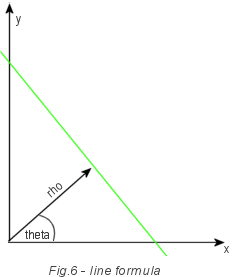
\includegraphics[width=0.5\textwidth]{inc/raster/design2-5.png}
  \caption{Угол поворота}
  \label{fig:fig25}
\end{figure}

Важным является то, что линия может быть описана всего двумя переменными: углом наклона и расстоянием до центра координат. 

Алгоритм проходит по всем пикселям в монохромном изображении, пропуская белые пиксели. Когда он попал на чёрный пиксель, то пытается «нарисовать» всевозможные линии, проходящие через этот пиксель с шагом в 1 градус. Это означает, что каждый пиксель имеет 180 воображаемых линий, проходящих через него, потому что углы 180-360 являются копиями линий с углами 0-180 градусов. 

Это множество воображаемых линий называется накопителем, двумерным массивом с размерностями $\theta$ и $rho$, которые были в формуле выше. Каждая воображаемая линия представлена одним значением в накопителе. Кстати, метод называется преобразованием, потому что он преобразовывает линии из $(x, y)$ в массив $(\theta, rho)$. Каждая воображаемая линия добавляет значение в накопитель, повышая вероятность того, что воображаемая линия совпадает с реальной. По аналогии с голосованием. Настоящие линии имеют больше всего «голосов». 

После того, как все пиксели и их 180 воображаемых линий «проголосовали», мы должны найти максимальное значение в накопителе. (Накопителем он называется потому что накапливает голоса) Победителем голосования является самая выразительная линия. Её параметра $\theta$ и $rho$ могут использоваться с помощью формулы выше чтобы нарисовать её. 

На следующем риc.~\ref{fig:fig26} приведён небольшой пример. Слева мы имеем линию, состоящую из трёх пикселей. Вы точно знаете, что это диагональная линия слева направо, но для компьютера это не так очевидно. 
\begin{figure}[ht!]
  \centering
  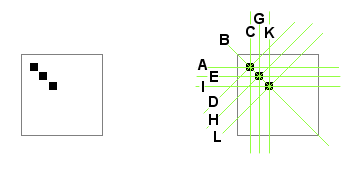
\includegraphics[width=0.6\textwidth]{inc/raster/design2-6.png}
  \caption{Определение нужной линии}
  \label{fig:fig26}
\end{figure}

Посмотрев на это изображение, можно понять, как же работает обнаружение линий. Алгоритм преобразования Хафа пропускает белые пиксели. На каждом чёрном пикселе он рисует четыре воображаемых зелёных линии (на самом деле их 180, но для простоты мы возьмём четыре), проходящие через текущий пиксель. Первый пиксель голосует за линии $A$, $B$, $C$ и $D$. Второй пиксель голосует за линии $E$, $B$, $G$, $H$. Третий за $I$, $B$, $K$, $L$. За линию $B$ проголосовали все три пикселя, а остальные линии получили всего по одному голосу. Таким образом, линия $B$ победила в голосовании.

\begin{figure}[ht!]
  \centering
  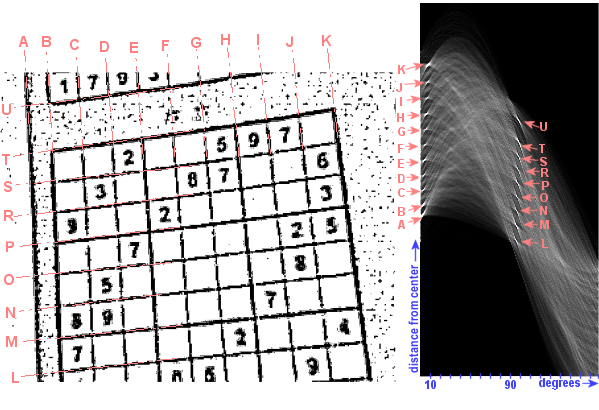
\includegraphics[width=0.8\textwidth]{inc/raster/design2-7.png}
  \caption{"Голосование" за линию}
  \label{fig:fig27}
\end{figure}
Следующий риc.~\ref{fig:fig27} является более сложным примером. Слева мы видим сетку судоку, а справа массив накопителя после прохождения по изображению алгоритма преобразования Хафа. Яркие светлые области являются линиями, которые получили много голосов. Темнота означает, что у нас нет шанса найти линию с такими параметрами на изображении. Сконцентрируемся только на ярких точках. Каждая линия $A-U$ имеет яркую точку в накопителе. Вы можете видеть, что все линии слегка повёрнуты (примерно на 6 градусов). Линия $A$ меньше повёрнута, чем линия $К$. Потому что изображение не только повёрнуто, но и скошено. Также, если вы посмотрите внимательнее, то увидите, что линии $А$ и $В$ ближе друг к другу, чем $В$ и $С$. Это можно заметить на обоих изображениях.

Преобразование Хафа важно понять, если вы хотите заниматься распознаванием образов. Концепция виртуальных линий, которые могут быть реальными с помощью голосования, может быть распространена на любую геометрическую фигуру. Линия – простейшая из них, поэтому является самой простой для понимания. 

Если вам надо найти окружность, то понадобится накопитель с тремя размерностями: $x$, $y$ и $r$. Где $x$ и $y$ являются координатами центра нашей окружности, а $r$ радиусом.

Преобразование Хафа может быть оптимизировано ограничением области и возможных углов исходного изображения. Нам не надо анализировать все линии, только те, что близки к центру. В нашем случае, именно от них мы и можем отталкиваться.

\subsubsection{Определение сетки}

Для получения чисел из сетки судоку, нам надо определить, а где же наша сетка начинается и кончается. Эта часть является простейшей частью для человеческого мозга, но самой сложной для автоматического распознавания. Почему? Почему бы не использовать линии, найденные с помощью преобразования Хафа в предыдущем шаге? В них слишком много лишних данных. На изображении будет слишком много лишних линий. 

Пример можно увидеть, посмотрев на риc.~\ref{fig:fig28}.
\begin{figure}[ht!]
  \centering
  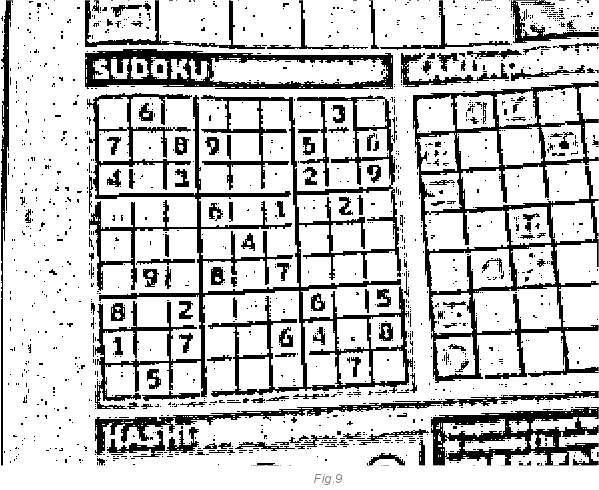
\includegraphics[width=0.8\textwidth]{inc/raster/design2-8.png}
  \caption{Зашумленное изображение}
  \label{fig:fig28}
\end{figure}

При автоматическом распознавании очень сложно определить, какие линии относятся к необходимым нам, а какие являются всего лишь информационным шумом. Где конец нашей сетки и начало следующей.

\begin{figure}[ht!]
  \centering
  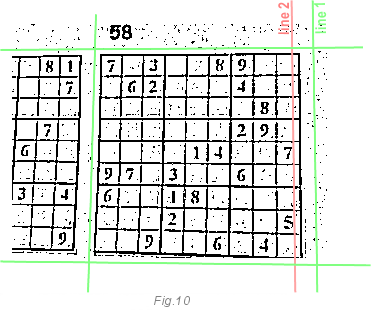
\includegraphics[width=0.8\textwidth]{inc/raster/design2-9.png}
  \caption{Отбрасывание информационного шума}
  \label{fig:fig29}
\end{figure}

Чтобы решить эту проблему, мы не будем определять чёрные линии. Вместо этого, мы будем определять белые области вокруг сетки. На  риc.~\ref{fig:fig29}, вы можете увидеть это. Зелёная линия 1 никогда не пересекается с чёрными пикселями в то время, как линия 2 делает это 10 раз. Это означает, что за сеткой скорее находится линия 1, нежели линия 2. Просто подсчитав, сколько раз зелёная линия пересекает чёрные пиксели, мы можем сделать вывод, что она находится за границей сетки. Достаточно просто подсчитать как много переходов с белого на чёрный пиксель под линией. Кстати, вам не надо пробегаться по каждой линии, достаточно выполнять эти действия каждую третью линию для увеличения скорости выполнения.


После того, как мы определили границы, запустим алгоритм преобразования Хафа чтобы точно определить линии сетки. До сих пор мы не заботились о перекосах и других дефектах изображения. Только об угле поворота. Этот шаг исправит это. Путём запуска преобразования Хафа, мы получим точные положения линий сетки. Это поможет определить числа в сетке.

Этот шаг может быть более устойчивым к шуму.

\subsection{Модуль OCR}
После того, как мы определили, где должны находиться числа, нам необходимо распознать их. Это относительно легко. В алфавите только цифры от 1 до 9.

Теория. Каждый алгоритм распознавания имеет три шага:
\begin{enumerate}
  \item определение необходимых признаков;
  \item тренировка;
  \item классификация (распознавание в реальности).
\end{enumerate}

Определение необходимых признаков является частью разработки приложения. Например, цифра один тонкая и высокая. Именно это и отличает её от остальных. Цифра 8 имеет две окружности, в верхней половине и в нижней, и т. д. 

Определение необходимых признаков может быть трудной и не интуитивной работой, в зависимости от того, что надо распознать. Например, что необходимо для распознавания чьего-то лица? Не любого, а какого-то конкретного.

\subsubsection{Зоны}
В нашем приложении был использован способ плотности зон. Следующим шагом (Это должно быть сделано заранее) является тренировка приложения на цифры от 1 до 9. Образцы эти изображения в каталоге хранятся в системе. Они уменьшены до размера 5х5, нормализованы и хранятся в статическом массиве \Code{OCRDigit[10]}, который выглядит примерно так как на рис.~\ref{fig:fig210}:

\begin{figure}[ht!]
  \centering
  
\includegraphics[width=\textwidth]{inc/raster/design2-10.png}
  \caption{Нормализованные и уменьшенные образцы изображений}
  \label{fig:fig210}
\end{figure}

Уменьшение до размеров 5х5 называется зоннированием или разбивкой на зоны. Массив выше называется плотностью функции.
Нормализация значит, что плотность варьируется от 0 до 1024. Без нормализации зоны нельзя сравнивать корректно.

Что происходит во время выполнения программы: когда цифра получена из исходного изображения, она уменьшается до размера 5х5. После этого каждый её пиксель сравнивается с каждым пикселем из девяти цифр из тренированного массива. Целью является найти цифру с минимальным различием. 

\begin{figure}[ht!]
  \centering
  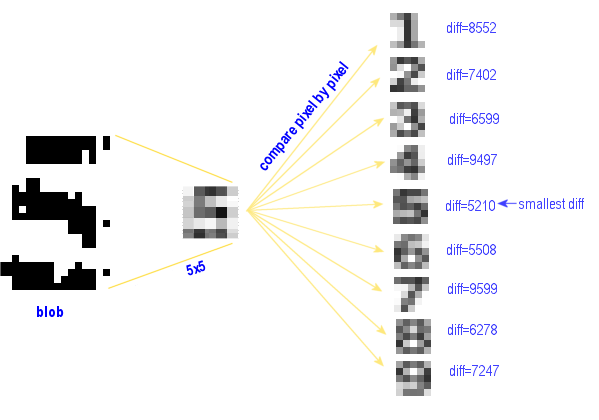
\includegraphics[width=\textwidth]{inc/raster/design2-11.png}
  \caption{Процесс уменьшения и сравнения с образцом}
  \label{fig:fig211}
\end{figure}
Этот метод инвариантен к размеру изображения, так как в любом случае мы используем зоны 5х5. Он чувствителен к поворотам, но мы уже позаботились об этом раньше. Проблема в том, что он чувствителен к позиции и смещению, а также не работает с негативами (белым по чёрному) и перевёрнутыми вверх тормашками цифрами. Изображен на на рис.~\ref{fig:fig211}

\subsubsection{Соотношение ширина/высота}

\begin{figure}[ht!]
  \centering
  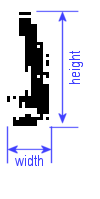
\includegraphics[width=0.1\textwidth]{inc/raster/design2-12.png}
  \caption{Пример цифры 1}
  \label{fig:fig212}
\end{figure}
Цифра один на ~\ref{fig:fig212} является частным случаем . Так как она похожа на 4 и 7, то метод определения, данный выше, может оказаться ненадёжным. Специфичный параметр единицы: в нашем случае, её ширина на 40\% меньше, чем высота. Нет другой такой цифры с таким же соотношением. У нас уже есть 25 зон (признаков), так вот это является 26-м признаком.

\begin{figure}[ht!]
  \centering
  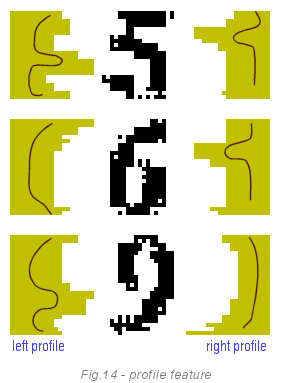
\includegraphics[width=0.5\textwidth]{inc/raster/design2-13.png}
  \caption{Пример цифры 1}
  \label{fig:fig212}
\end{figure}
Качество OCR может быть улучшено введением новых признаков. Например, цифры 5,6 и 9 очень похожи при использовании разбиения на зоны. Для того, чтобы различать их, мы можем использовать их профили как признаки. Особенностью признака является количество пикселей (расстояние) между краем рамки цифры и её границей.

На изображении ниже, вы можете видеть, что профили цифр 5 и 6 похожи, но они отличаются от профиля 9. Левый профиль 5 и 9 похож, но отличается от профиля 6.

\subsubsection{Корректировка результатов OCR}

Как только OCR закончен, результаты корректируются в соответствии с правилами судоку. 

В одной строке, столбце и блоке 3х3 не может находиться одна и та же цифра. Если правило нарушено, то необходимо ввести коррективы в полученные результаты. Мы заменим неправильную цифру той, что возможна из оставшихся. 

Например, на рис.~\ref{fig:fig211} выше, результат 5 потому что $diff = 5210$, которое является самым маленьким значением различия. Следующий возможный результат $6$, так как $diff = 5508$ в этом случае. Таким образом, мы заменим $5$ на $6$. Чтобы решить, которая из двух цифр неверная, мы сравним значения их различий с их образцами, и та, у которой значение меньше, будет считаться верной. 

\subsection{Принцип работы системы}
 Область распознавания изображений является одной из самых захватывающих в современных компьютерных вычислениях, и она очень сложна. Что легко и просто для человеческого мозга, то очень сложно для системы. Многие вещи до сих пор остаются невозможными с сегодняшним уровнем развития IT.

На блок-схеме на рис.~\ref{fig:fig211} представлены все этапы, которые проходит изображение перед тем, как будет распознано.
\begin{figure}[ht]
  \centering
  \includegraphics[width=0.3\textwidth]{inc/dia/design2-14}
  \caption{Блок-схема подсистемы распознавания}
  \label{fig:fig214}
\end{figure}

После распознавания мы сохраняем результаты в CSV-файл.

Для обмена данными между роботом и мобильным устройством будем использовать формат CSV.

\paragraph{CSV} (от англ. Comma-Separated Values — значения, разделённые запятыми) — текстовый формат, предназначенный для представления табличных данных. Каждая строка файла — это одна строка таблицы. Значения отдельных колонок разделяются разделительным символом (delimiter) — запятой (,). Однако, большинство программ вольно трактует стандарт CSV и допускают использование иных символов в качестве разделителя. 

Пример распознанного изображения в формате CSV:
\begin{lstlisting}[caption=CSV файл с заданием]
5,3,,,7,,,,
6,,195,,
,9,8,,,,6,
8,,,6,,,,3
4,,8,,3,,1
7,,,2,,,6
,6,,,,,2,8,
,,,4,1,9,,,5
,,,,8,,,7,9
\end{lstlisting}

Нас данный вариант устраивает, так формат достаточно компактен для передачи и нам не нужно "захлямлять" информационным шумом потоки передачи данных. 

\section{Подсистема передачи данных}

Нашей наиболее часто выполняемой задаче будет передача распознанного CSV-файла с мобильного телефона на контроллер робота.

В листинге~\ref{lst:analyt1} и листинге~\ref{lst:analyt2} приведены примеры обмена данными между роботом и телефоном, описанные в протоколе сообщений робота.

Процесс сопряжения мы можем произвести с помощью встроенных возможностей каждого из устройств, поэтому дублировать его не имеет смысла и воспользуемся стандартной процедурой сопряжения.

\subsection{Обмен данными между устройствами}

У нас есть список команд, описание протокола, сформированный файл, но проблема в том, что у нас лимит сообщения 64 байта.

Нам неудобно разрывать файл, управляющие команды и остальные сообщения на большое количество частиц.

Для этого мы воспользуемся \textbf{Bluetooth сокетами}.

\paragraph{Bluetooth сокет} -  API, позволяющий реализовывать взаимодействие между узлами или между процессами на одном узле. Данная технология может работать со множеством различных устройств ввода-вывода и драйверов, несмотря на то, что их поддержка зависит от реализации операционной системы.

С мобильного устройства у нас будут отправляться данные, а на роботе будут приниматься.

На телефоне мы создаем отправляющий сокет, приведенный в листинге~\ref{lst:design1} 

\begin{lstlisting}[caption={Создаем сокет с данными для отправки}, label=lst:design1, language=Java]
Method m = device.getClass().getMethod("createRfcommSocket", new Class[] { int.class }); 
BluetoothSocket sendSocket = (BluetoothSocket) m.invoke(device, 1);
\end{lstlisting}

На роботе в свою очередь, для работы мы будем использовать тип \textbf{Message Write} и \textbf{Message Read}, который позволяет обмениваться произвольными сообщениями между устройствами в текстовом виде, а дальнейшая обработка ляжет уже на контроллер робота и второе устройство обмена.

Наша задача состоит в том, чтобы 
\begin{enumerate}
  \item открыть/создать сокет;
  \item обменяться данными;
  \item закрыть сокет (зафиксировав файл на конечном устройстве).
\end{enumerate}

Выполнил эти три простые операции, мы гарантируем отправку и доставку данных. Причем целостность данных, как на уровне файлов, так и на уровне пакетов будут лежать уже на сокетах.

Сокеты поддерживаются обоими устройствами и API-робота дает нам возможность принимать данные.

\subsection{Прием и отправка данных с мобильного устройства}

Наше устройство под управлением ОС Android будет обмениваться данными с роботом.

Помимо файла с заданием мы будем получать от робота еще и некоторую диагностическую информацию.

Дело в том, что в Android'е для приема данных от какого-либо устройства необходимо создавать отдельный фоновый поток, чтобы у нас не зависало основное активити. Для этого мы задействуем thread и все данные будут приниматься в отдельном потоке.

Для работы с Bluetooth нам необходимо будем минимум 3 библиотеки, не считая Java-библиотек для работ с потоками:
\begin{lstlisting}[caption={Библиотеки для работы с Bluetooth на ОС Android}, label=lst:design2, language=Java]
import android.bluetooth.BluetoothAdapter;
import android.bluetooth.BluetoothDevice;
import android.bluetooth.BluetoothSocket;
\end{lstlisting}

Первая библиотека в листинге~\ref{lst:design1},  позволяет нам работать с нашим Bluetooth-адаптером, например проверить включен ли, получить адаптер через который будем работать и другие операции.

Вторая библиотека позволяет нам работать с устройствами Bluetooth, такие операции как получение удаленного устройства, получить операции с сокетами и другие.

Ну и третья библиотека для работы с сокетами, принцип работы которых был описан чуть выше.

Модуль на мобильном устройстве должен работать в двух режимах: должен отправлять задание и слушать порт, чтобы получать диагностическую информацию.

Диаграмма последовательности обмена сообщениями приведена на на рис~\ref{fig:fig25}
\begin{figure}[ht!]
  \centering
  \includegraphics[width=\textwidth]{inc/dia/design2-18}
  \caption{Диаграмма последовательности обмена сообщениями}
  \label{fig:fig25}
\end{figure}


\subsection{Прием и отправка данных с контроллера робота}

Для работы с роботом нам предоставлено упрощенное API для работы с устройствами семейства Bluetooth.

У нас есть всего одно пространство имен:
\begin{lstlisting}[caption={Пространство для работы с Bluetooth на контроллерах NXT}, label=lst:design3]
javax.bluetooth
\end{lstlisting}

И всего 4 класса, которые предоставляют весь нам необходимый функционал:
\begin{lstlisting}[caption={Классы для работы с Bluetooth на контроллерах NXT}, label=lst:design4]
DeviceClass 
DiscoveryAgent 
LocalDevice 
RemoteDevice
\end{lstlisting}

Первый класс предоставляем нам возможности стандартной спецификации Bluetooth и по большому мало применим.

Второй класс предоставляем нам весь набор команд и возможностей для обмена данными и прочей обработки, возвращается как парамет при вызове некоторых методов из \Code{LocalDevice} и \Code{RemoteDevice}. То есть этот класс набор инструкций. 

И последние 2 класса нам нужны для работы с локальным устройством Bluetooth, в нашем случае с устройстом контроллера и удаленным устройством.

Наша задача состоит в том, чтобы RemoteDevice принял данные, отправленные через наш сокет и принялся их решать.

\subsection{Обмен диагностической информацией}

Чтобы мы могли узнать успешно ли прошла операция, сколько времени на нее затратилось, какое решение имеет то или иное задание, мы будем использовать диагностическую информацию приведенную в данном разделе.

Во-первых, чтобы не отправлять постоянной файлик с заданием, мы применим для него хеш-функцию MD5.

\paragraph{MD5 (англ. Message Digest 5)} — 128-битный алгоритм хеширования.

Хеш содержит 128 бит (16 байт) и обычно представляется как последовательность из 32 шестнадцатеричных цифр. На ~\ref{lst:design5},

\begin{lstlisting}[caption={Пример MD5 хеша}, label=lst:design5]
MD5("md5") = 1bc29b36f623ba82aaf6724fd3b16718
\end{lstlisting}

Мы будем брать MD5 хеш от задания, что не передавать каждый раз задание целиком.

Информация, которая нам необходимо собирать в процессе решения:
\begin{enumerate}
  \item фотография, которая соответствует заданию;
  \item само задание;
  \item статус решено или нет;
  \item время решения;
  \item ответ.
\end{enumerate}

Последние 3 пункта мы получаем с робота.

Для идентификации заданий, мы будем хешировать каждое задание и будем индексировать его по значению его хеша.

Схему базы данных можно посмотреть на рис~\ref{fig:fig24}
\begin{figure}[ht!]
  \centering
  \includegraphics[width=\textwidth]{inc/dia/design2-17}
  \caption{ER диаграмма}
  \label{fig:fig24}
\end{figure}


У нескольких фотографий может быть один и тот же хеш, так же необходимо учесть, что у одного задания может быть несколько решений, при плохо спроектированном задании Судоку.

\section{Подсистема решения}

Так для подсистемы определили, что скорость решения одна из существенных характеристик для данной подсистемы, мы будем использовать комбинацию из 

\begin{enumerate}
  \item метода перебора;
  \item метода открытых пар;
  \item метода скрытых пар.
\end{enumerate}

Перебор не слишком быстрый метод. Методы открытых  и скрытых пар очень быстрые, но могут решать только быстрые пазлы. Так как мы просим приложение решить пазл за нас, то это значит, что он действительно сложный. 

Наша подсистема должна решать любые пазлы, поэтому скомбинируем решение методов в такой последовательности:

\begin{enumerate}
  \item метод открытых пар;
  \item метод скрытых пар;
  \item метод перебора.
\end{enumerate}

В начале расположены два быстрых метода, и только если им не удаётся решить пазл, управление переходит к решению методом перебора, уменьшив работу для этого алгоритма. 

Ниже на рис.~\ref{fig:fig23} приведён алгоритм работы. 


\begin{figure}[ht!]
  \centering
  \includegraphics[height=0.95\textheight]{inc/dia/design2-16}
  \caption{Блок-схема алгоритма решения}
  \label{fig:fig23}
\end{figure}

Только если методы открытых и скрытых пар не могут решить пазл, программа начинает передирать значения. И даже тогда, алгоритм перебора ограничен по времени 600000 итерациями. Также существует три попытки, после чего программа сдаётся. Между каждой попыткой, рекурсивная последовательность переставляется случайным образом с надеждой, что новая последовательность поможет решить пазл быстрее. 










